\documentclass[11pt]{amsart}

% Include Packages
\usepackage{amsfonts}
\usepackage{amsmath}
\usepackage{amssymb}
\usepackage{amsthm}
\usepackage{amsxtra}
\usepackage{caption}
\usepackage{epsfig,color}
\usepackage{enumerate}
\usepackage[dvipsnames]{xcolor}
\usepackage{fullpage}
\usepackage{hyperref}
\usepackage{mathtools}
\usepackage{vmargin}
\usepackage{MnSymbol}
% Tikz package and libraries
\usepackage{tikz}
\usepackage{tikz-cd}
%\usepackage{tikzducks}
\usetikzlibrary{arrows, backgrounds, chains, decorations.pathreplacing, patterns, shapes, calc, positioning}

% Theorem Commands
\theoremstyle{plain}
\newtheorem{theorem}{Theorem}[section]
\newtheorem{corollary}[theorem]{Corollary}
\newtheorem{lemma}[theorem]{Lemma}
\newtheorem{proposition}[theorem]{Proposition}
\newtheorem*{claim}{Claim}
\newtheorem{conjecture}{Conjecture}

\theoremstyle{definition}
\newtheorem{definition}{Definition}
\newtheorem*{question}{Question}
\newtheorem*{notation}{Notation}
\newtheorem{exercise}{Exercise}

\theoremstyle{remark}
\newtheorem{remark}{Remark}[section]
\newtheorem{example}{Example}[section]
\newtheorem{examples}{Examples}

\newcommand{\RR}{\mathbb{R}}
\newcommand{\LL}{\mathcal{L}}
\newcommand{\CC}{\mathbb{C}}
\newcommand{\ZZ}{\mathbb{Z}}
\newcommand{\NN}{\mathbb{N}}

\DeclareMathOperator{\id}{id}
\DeclareMathOperator{\Des}{Des}
\DeclareMathOperator{\maj}{maj}


\newcommand{\binomsq}[2]{\left[\begin{matrix} #1 \\ #2 \end{matrix}\right]}

\numberwithin{equation}{section}

\setmarginsrb{33mm}{30mm}{33mm}{40mm}%
            {0mm}{10mm}{0mm}{10mm}


\begin{document}

\begin{center}
	\huge{Algebraic combinatorics}
\end{center}

\bigskip

\begin{center}
	\Large{Lecture 17: The Fundamental Lemma of $(P, w)$-partitions (20/11/2025)}
\end{center}

\bigskip

\begin{center}
	\Large{Michele D'Adderio}
\end{center}
\smallskip
\begin{center}
	\large{(notes by Gabriel Antonio Videtta)}
\end{center}
\bigskip
\begin{center}
	\textcolor{red}{
		WARNING: any information contained in these notes can be wrong!}\\
	\textcolor{red}{READER DISCRETION IS ADVISED}
\end{center}

\tableofcontents

\section{Labelled posets and \texorpdfstring{$(P, w)$}{(P, w)}-partitions}

We're looking to find a suitable statistic to associate to $\Omega(P, n)$,
the order-reversing\footnote{
	This is merely a convention. The theory concerning order-preserving maps is
	studied using essentially the same arguments, with appropriate adjustments.
} functions from a poset $P$ to a chain of length $n$ (e.g., $\{1 \leq 2 \leq \cdots \leq n\}$). \medskip

As a first approach, we will define a generating function tracking \textit{every} aspect of such functions,
and we will restrict ourselves to a more particular statistic in the future lectures.

In order to do so, we will assume we have a fixed \textit{labelling} $w$ for our poset $P$:

\begin{definition}
	Let $P$ be a poset with $n$ elements. A \textit{labelling of $P$} is a bijection $w : P \to [n]$.
\end{definition}

\begin{figure}[h]
	\centering
	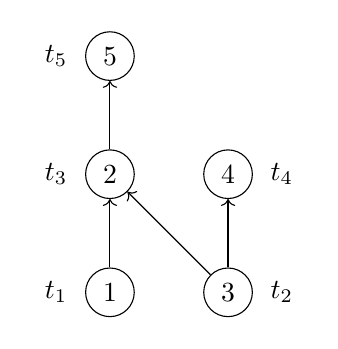
\begin{tikzpicture}
		\begin{scope}[every node/.style={circle,draw}]
			\node (A) at (0,0) [label=left:$t_1$] {1};
			\node (B) at (1.5,0) [label=right:$t_2$] {3};
			\node (C) at (0,1.5) [label=left:$t_3$] {2};
			\node (D) at (1.5,1.5) [label=right:$t_4$] {4};
			\node (E) at (0,3) [label=left:$t_5$] {5};
		\end{scope}

		\draw[->] (A) -- (C);
		\draw[->] (B) -- (C);
		\draw[->] (B) -- (D);
		\draw[->] (C) -- (E);

	\end{tikzpicture}
	\caption{A \textit{labelled} poset $\{t_1, t_2, t_3, t_4, t_5\}$, with
		$t_1$, $t_2 \leq t_3 \leq t_5$ and $t_2 \leq t_4$. The labels are represented within
		the circled nodes.}
	\label{fig:example_labelled_poset}
\end{figure}

We are now ready to state the definition for a $(P, w)$-partition, which allows us to be more flexible on
the choice of the ``weaknesses'' of our order-reversing maps:

\begin{definition}
	A $(P, w)$-partition is a map $\sigma : P \to \NN$ with the following two properties:

	\begin{enumerate}[(i.)]
		\item \textit{it's (weakly) order-reversing:} if $s <_P t$, then $\sigma(s) \geq \sigma(t)$;
		\item \textit{it respects the strictness according to the labelling:} if $s <_P t$ and
		      $w(s) > w(t)$, then $\sigma(s) > \sigma(t)$.
	\end{enumerate}
\end{definition}

\begin{notation}
	We will denote the set of all $(P, w)$-partitions of $P$ with $A(P, w)$.
\end{notation}

\begin{example}
	For Figure \ref{fig:example_labelled_poset}, the resulting conditions for a map $\sigma$ to be
	a $(P, w)$-partition are:
	\begin{itemize}
		\item being (weakly) order-reversing;
		\item $\sigma(t_2) > \sigma(t_3)$, since $t_2 < t_3$ and $w(t_2) = 3 > 2 = w(t_3)$.
	\end{itemize}
\end{example}

\begin{remark}
	If we choose a labelling $w$ such that, whenever $s <_P t$, $w(s) < w(t)$, a $(P, w)$-partition is
	simply an order-reversing map -- it must satisfy only (i.), since (ii.) is vacuously true.

	Likewise, if we choose $w$ such that $w(s) > w(t)$, then the map must be \textit{strictly} order-reversing.
\end{remark}

These observations lead us to the following definitions:

\begin{definition}
	We say a labelling $w$ is \textit{natural} if, whenever $s <_P t$, $w(s) < w(t)$. We say $w$ is \textit{dually natural} if
	$w(s) > w(t)$ whenever $s <_P t$. \smallskip
\end{definition}

For (dual) natural labellings, the conditions for a map to be $(P, w)$-partition do not depend on $w$. Therefore they are simply
called (strict) $P$-partitions. \smallskip

We are now ready to define a statistics on the $(P, w)$-partitions:

\begin{definition}
	Let $P = \{t_1, t_2, \ldots, t_n\}$ be a poset with labelling $w$. We then define the \textit{$(P, w)$-partition enumerator} as:
	\[
		F_{P, w} \coloneq F_{P, w}(x_1, \ldots, x_n) \coloneq \sum_{\sigma \in A(P, w)} x_1^{\sigma(t_1)} \cdots x_n^{\sigma(t_n)}.
	\]
\end{definition}

\begin{remark}
	Given a natural labelling $w$, the generating function $F_{P, w}$ enumerates all the order-reversing maps from the $\Omega(P, n)$'s. To restrict
	to a certain $n$, we simply ignore any monomials that contain a variable with degree greater than $n$.
\end{remark}

The following examples provide insight into why the $(P, w)$-partition enumerator, in a certain sense, generalizes the partitions we've studied on the integers.

\begin{example} \label{ex:chain_n}
	Let $P$ be a naturally labelled chain $t_1 < t_2 < \cdots < t_n$. Recall that in this case a $P$-partition is the same as an order-reversing map. Thus:
	\[
		F_P = \sum_{a_1 \geq a_2 \geq \cdots a_n \geq 0} x_1^{a_1} \cdots x_n^{a_n} = \frac{1}{(1-x_1) (1-x_1 x_2) \cdots (1 - x_1 x_2 \cdots x_n)}.
	\]
\end{example}

\begin{example}
	Let $P$ be a dually naturally labelled chain $t_1 < t_2 < \cdots < t_n$. In this case a $P$-partition is the same as a \textit{strict} order-reversing map.
	Therefore:
	\[
		F_P = \sum_{a_1 > a_2 > \cdots a_n > 0} x_1^{a_1} \cdots x_n^{a_n} = \frac{x_1^{n-1} x_2^{n-2} \cdots x_{n-1}}{(1-x_1) (1-x_1 x_2) \cdots (1 - x_1 x_2 \cdots x_n)}.
	\]
\end{example}

\begin{example} \label{ex:antichain_n}
	Let $P$ be an antichain (i.e., no comparisons are possible) of size $n$. It is a simple \textbf{exercise} to check that
	$(P, w)$-partitions do not depend on $w$ and are simply maps from $P$ to $\NN$. Hence:
	\[ F_P = \frac{1}{(1-x_1) \cdots (1-x_n)}. \]

	\begin{remark}
		$F_P$ enumerates, in a certain sense, the possible partitions on $[n]$. Choosing $x_i = x^i$, we get the \textit{partition enumerator} series.
	\end{remark}
\end{example}

\begin{notation}
	Let $P$ be a poset of size $n$ with labelling $w$.
	We will employ the notation $\LL(P, w)$ to denote the set of permutations $\pi = \pi_1 \cdots \pi_n \in S_n$ such that the map $\sigma : P \to [n]$ defined
	by $\sigma(w^{-1}(\pi_i)) = i$ is a linear extension (i.e., an order-preserving map) of $P$.
\end{notation}

\begin{remark}
	Let $P = [n]$ be a poset. There is a natural labelling on $P$, namely the identity map $\id \in S_n$. This simplifies
	the definition of $\LL(P, w)$:

	\vspace{0.1in}

	\begin{quote}
		$\LL(P, w)$ is the set of permutations $\pi = \pi_1 \cdots \pi_n \in S_n$ such that the map $\sigma : P \to [n]$ defined
		by $\sigma(\pi_i) = i$ is a linear extension (i.e., an order-preserving map) of $P$.
	\end{quote}

	\vspace{0.1in}

	In other words:

	\vspace{0.1in}

	\begin{quote}
		$\LL(P, w)$ is the set of permutation $\pi \in S_n$ such that if $i \leq_P j$, then $i$ comes before $j$ in
		the one-line notation of $\pi$.
	\end{quote}
\end{remark}

\begin{example}
	\begin{figure}[h]
		\centering
		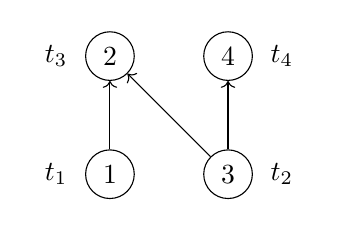
\begin{tikzpicture}
			\begin{scope}[every node/.style={circle,draw}]
				\node (A) at (0,0) [label=left:$t_1$] {1};
				\node (B) at (1.5,0) [label=right:$t_2$] {3};
				\node (C) at (0,1.5) [label=left:$t_3$] {2};
				\node (D) at (1.5,1.5) [label=right:$t_4$] {4};
			\end{scope}

			\draw[->] (A) -- (C);
			\draw[->] (B) -- (C);
			\draw[->] (B) -- (D);

		\end{tikzpicture}
		\caption{A \textit{labelled} poset $\{t_1, t_2, t_3, t_4\}$, with
			$t_1$, $t_2 \leq t_3$ and $t_2 \leq t_4$. The labels are represented within
			the circled nodes.}
		\label{fig:example_Lpw}
	\end{figure}

	Let's compute $\LL(P, w)$ for the labelled poset from Figure \ref{fig:example_Lpw}.
	$1$ and $3$ must come before $2$; $3$ must come before $4$ as well. Therefore:
	\[ \LL(P, w) = \{ 1324, 1342, 3124, 3142, 3412 \}. \]
\end{example}

\section{\texorpdfstring{$\pi$}{π}-compatibility and the Fundamental Lemma of \texorpdfstring{$(P, w)$}{(P, w)}-partitions}

\begin{definition}
	Let $\pi$ be a permutation of $n$ elements. A function $f : [n] \to \NN$ is said to be \textit{$\pi$-compatible} if:

	\begin{itemize}
		\item \textit{it weakly decreases along the one-line notation of $\pi$:} $f(\pi_1) \geq f(\pi_2) \geq \cdots \geq f(\pi_n)$.
		\item \textit{strictness is forced upon a descent:} $f(\pi_i) > f(\pi_{i+1})$ if $i$ is a descent (i.e., if $\pi_i > \pi_{i+1}$).
	\end{itemize}
\end{definition}

\begin{lemma}
	Let $f$ be a function from $[n]$ to $\NN$. Then, there exists a unique permutation $\pi \in S_n$ such that
	$f$ is $\pi$-compatible. \label{lem:unique_pi_permutation}
\end{lemma}

\begin{proof}
	Consider the unique (\textbf{exercise}) ordered set partition $(B_1, B_2, \ldots, B_k)$ such that
	$f \big|_{B_i}$ is constant and $f \big|_{B_1} > f \big|_{B_2} > \cdots > f \big|_{B_k}$. (continue)
	\begin{example}
		Let $f : [5] \to \NN$ be such that:

		\begin{itemize}
			\item $f(2) = f(3) = 1$;
			\item $f(1) = f(4) = 6$;
			\item $f(5) = 8$.
		\end{itemize}

		Thus, $B_1 = \{5\}$, $B_2 = \{1, 4\}$ and $B_3 = \{2, 3\}$, since $8 > 6 > 1$.
	\end{example}

	We are now ready to construct our permutation $\pi$ by specifying its one-line notation.
	First, we order the elements within each block $B_i$ in increasing order:
	\[
		B_i = \{ b_{i,1} \leq b_{i,2} \leq \cdots \leq b_{i, j_i} \}.
	\]
	We then define $\pi$ by concatenating these ordered blocks:
	\[
		\pi = b_{1,1} \cdots b_{1, j_1} b_{2,1} \cdots b_{2, j_2} \cdots b_{k, j_k}.
	\]
	One can verify that $f$ is indeed $\pi$-compatible (\textbf{exercise}). The uniqueness of the permutation
	$\pi$ follows straightforwardly from the uniqueness of the set partition $(B_1, B_2, \ldots, B_k)$.
\end{proof}

\begin{definition}
	Let $\sigma$ be a map from $P$ to $\NN$, where $(P, w)$ is a labelled poset of size $n$. We then define
	the map $\sigma'$ from $[n]$ to $\NN$ to be the re-indexed version of $\sigma$ via $w$, where the label $w(p) \in [n]$
	is used instead of the poset element $p \in P$. In other words, $\sigma'$ is such that:
	\[
		\sigma'(i) = \sigma(w^{-1}(i)).
	\]
\end{definition}

\begin{notation}
	Let $(P, w)$ be a labelled poset of size $n$, and let $\pi \in S_n$ be a permutation of $n$ elements. We will employ the notation $S_\pi$
	to denote the set of all maps $\sigma$ from $P$ to $\NN$ such that their re-indexed versions $\sigma'$ are $\pi$-compatible.
\end{notation}

\begin{theorem}[Fundamental Lemma of $(P, w)$-partitions]
	The set of $(P, w)$-partitions $A(P, w)$ is exactly the disjoint union of the $S_\pi$'s, where $\pi$ varies over $\LL(P, w)$:
	\[
		A(P, w) = \bigsqcup_{\pi \in \LL(P, w)} S_\pi.
	\] \label{thm:fundamental_lemma}
\end{theorem}

\begin{proof}
	The disjointness of the right hand side follows straightforwardly from Lemma \ref{lem:unique_pi_permutation}.
	We now prove both inclusions.

	\begin{itemize}
		\item[($\subseteq$)] Let $\sigma \in A(P, w)$. Lemma \ref{lem:unique_pi_permutation} tells us there exists a unique
		      $\pi$ such that $\sigma \in S_\pi$. It remains only to verify that $\pi$ is an element of $\LL(P, w)$.

		      Let $\pi = \pi_1 \cdots \pi_n$. Suppose $i < j$, $w(s) = \pi_i$ and $w(t) = \pi_j$. We need to show that
		      $s \not> t$.

		      Since $\sigma \in S_\pi$, then:
		      \[ \sigma(s) = \sigma'(\pi_i) \geq \sigma'(\pi_j) = \sigma(t). \]
		      If we had $\sigma(s) > \sigma(t)$, then $s \not> t$, since $\sigma$ is order-reversing. Suppose then
		      $\sigma(s) = \sigma(t)$, i.e., $\sigma'(\pi_i) = \sigma'(\pi_j)$. Therefore we have:
		      \[
			      \pi_i < \pi_{i+1} < \cdots < \pi_j,
		      \]
		      since there cannot be descents (otherwise we'd have $\sigma(s) > \sigma(t)$, \textbf{exercise}). Thus
		      $w(s) = \pi_i < \pi_j = w(t)$: if we had $s > t$, we would have $\sigma(t) > \sigma(s)$, which contradicts
		      our supposition. It follows that $s$ cannot be greater than $t$, and then that $A(P, w) \subseteq \bigsqcup_{\pi \in \LL(P, w)} S_\pi$.

		\item[($\supseteq$)] Let $\sigma$ be a map from $P$ to $\NN$ such that $\sigma'$ is $\pi$-compatible, with $\pi \in \LL(P, w)$. We need to show
		      that $\sigma$ is an element of $A(P, w)$. We will do so by showing that $\sigma$ satisfies the two conditions for being a $(P, w)$-partition.

		      Let $s$, $t$ be elements of $P$ such that $s < t$. Let $\pi_i = w(s)$ and $\pi_j = w(t)$. Since
		      $\pi$ is an element of $\LL(P, w)$, then $\pi_i$ must come before $\pi_j$ in the one-line notation of $\pi$, i.e., $i < j$. Since $\sigma'$ is
		      $\pi$-compatible, we have $\sigma(s) = \sigma'(\pi_i) \geq \sigma'(\pi_j) = \sigma(t)$.

		      Suppose now that $w(s) > w(t)$. Then, $\pi_i$ is strictly bigger than $\pi_j$, meaning there exists a descent $k$ with $i \leq k < j$. Therefore:
		      \[
			      \sigma(s) = \sigma'(\pi_i) \geq \sigma'(\pi_{i+1}) \geq \cdots \geq \sigma'(\pi_k) > \sigma'(\pi_{k+1}) \geq \cdots \geq \sigma'(\pi_j) = \sigma(t).
		      \]
		      This concludes our proof.
	\end{itemize}
\end{proof}

The usefulness of the \nameref{thm:fundamental_lemma} comes from the fact that the generating function $F_{P, w}$ is easier to describe on $S_\pi$, as shown in the following result.

\begin{definition}
	Let $\pi \in S_n$ be a permutation of $n$ elements, and let $P = \{t_1, \ldots, t_n\}$ be a poset with size $n$ and labelling $w$. We then define a new
	permutation $\pi' \in S_n$, such that $\pi'$ gives the index of the element in $P$ corresponding to the value in $\pi$. Specifically, $\pi'$ is such that:
	\[
		\pi_i = w(t_j) \implies \pi_i' = j.
	\]
\end{definition}

\begin{lemma}
	Let $\pi \in S_n$ be a permutation of $n$ elements, and let $P = \{t_1, t_2, \ldots, t_n\}$ be a poset with size $n$ and labelling $w$. Then:
	\[
		F_{P, w, \pi} \coloneq \sum_{\sigma \in S_\pi} x_1^{\sigma(t_1)} \cdots x_n^{\sigma(t_n)} = \frac{\prod_{j \in \Des(\pi)} x_{\pi_1'} x_{\pi_2'} \cdots x_{\pi_j'}}{\prod_{i=1}^n (1 - x_{\pi_1'} \cdots x_{\pi_i'})}.
	\] \label{lem:F_pi}
\end{lemma}

\begin{proof}
	\underline{This part is happily left to the professor to fill.}
\end{proof}

As an immediate application of Lemma \ref{lem:F_pi} and the \nameref{thm:fundamental_lemma}, we get the following theorem (\textbf{exercise}):

\begin{theorem}
	Let $P = \{t_1, t_2, \ldots, t_n\}$ be a poset with size $n$ and labelling $w$. Then:
	\[
		F_{P, w} = \sum_{\pi \in \LL(P, w)} \frac{\prod_{j \in \Des(\pi)} x_{\pi_1'} x_{\pi_2'} \cdots x_{\pi_j'}}{\prod_{i=1}^n (1 - x_{\pi_1'} \cdots x_{\pi_i'})}.
	\] \label{thm:F_pw}
\end{theorem}

\section{Applications of the Fundamental Lemma}

Let's specialise the series from Theorem \ref{thm:F_pw} and get its $q$-analogue. We will denote
it with $F_{P, w}(q) := F_{P, w}(q, q, \ldots, q)$.

\begin{example}
	Let $P$ be a chain of size $n$ with a natural labelling. Thus $\LL(P, w)$ consists of only the identity $\id \in S_n$, with $\maj(\id) = 0$.
	Therefore: \label{ex:Fq_chain}
	\[
		F_P(q) = \frac{q^{\maj(\pi)}}{(1-q)(1-q^2) \cdots (1-q^n)} = \frac{1}{(1-q)(1-q^2) \cdots (1-q^n)},
	\]
	which is consistent with what we'd already seen in Example \ref{ex:chain_n}
\end{example}

The \nameref{thm:fundamental_lemma} and Theorem \ref{thm:F_pw} allow us to provide alternative
proofs for some of the theorems established in previous lectures.

\begin{example}
	Let $P$ be an antichain of size $n$. Thus $\LL(P, w) = S_n$. Using the results from Example \ref{ex:antichain_n}, we get:
	\[
		\frac{1}{(1-q)^n} = F_P(q) = \frac{\sum_{\pi \in S_n} q^{\maj(\pi)}}{(1-q)(1-q^2) \cdots (1-q^n)},
	\]
	from which the MacMahon theorem follows:
	\[
		\sum_{\pi \in S_n} q^{\maj(\pi)} = \prod_{i=1}^n \frac{1-q^i}{1-q} = \prod_{i=1}^n [i]_q = [n]_q ! \, .
	\]
\end{example}

\begin{example}
	Let $P = C_n + C_k$ be a disjoint union of two chains (see Figure \ref{fig:example_disjoint_union_two_chains}).

	\begin{figure}[h]
		\centering
		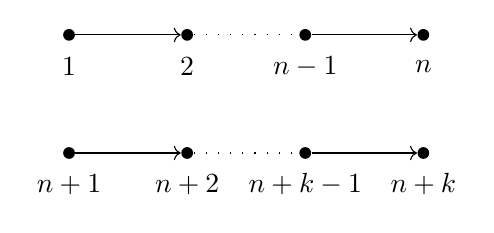
\begin{tikzpicture}
			% C_n
			\node[circle, fill, inner sep=1.5pt] (A) at (0,1.5) {};
			\node at (0, 1.1) {$1$};

			\node[circle, fill, inner sep=1.5pt] (B) at (1.5,1.5) {};
			\node at (1.5, 1.1) {$2$};

			\node[circle, fill, inner sep=1.5pt] (C) at (3,1.5) {};
			\node at (3, 1.1) {$n-1$};

			\node[circle, fill, inner sep=1.5pt] (D) at (4.5,1.5) {};
			\node at (4.5, 1.1) {$n$};

			% C_k

			\node[circle, fill, inner sep=1.5pt] (A1) at (0,0) {};
			\node at (0, -0.4) {$n+1$};

			\node[circle, fill, inner sep=1.5pt] (B1) at (1.5,0) {};
			\node at (1.5, -0.4) {$n+2$};

			\node[circle, fill, inner sep=1.5pt] (C1) at (3,0) {};
			\node at (3, -0.4) {$n+k-1$};

			\node[circle, fill, inner sep=1.5pt] (D1) at (4.5,0) {};
			\node at (4.5, -0.4) {$n+k$};

			\draw[->] (A) -- (B);
			\draw[loosely dotted] (B) -- (C);
			\draw[->] (C) -- (D);

			\draw[->] (A1) -- (B1);
			\draw[loosely dotted] (B1) -- (C1);
			\draw[->] (C1) -- (D1);

		\end{tikzpicture}
		\caption{The \textit{labelled} disjoint union of two chains, one of length $n$ and the other of length $k$.}
		\label{fig:example_disjoint_union_two_chains}
	\end{figure}

	One can easily verify (\textbf{exercise}) that:
	\[
		F_P(q) = F_{C_k}(q) \cdot F_{C_n}(q).
	\]
	Recall from Example \ref{ex:Fq_chain} that the following identity holds:
	\[
		F_{C_n}(q) = \prod_{i=1}^n \frac{1}{1-q^i}, \qquad F_{C_k}(q) = \prod_{j=1}^k \frac{1}{1-q^j}.
	\]
	We can identify $\LL(P)$ with words with $n$ $0$'s and $k$ $1$'s, with the zeros representing elements from $C_n$ and the
	ones representing elements from $C_k$ (\textbf{exercise}). Thus, by applying Theorem \ref{thm:F_pw} we get:
	\[
		\left( \prod_{i=1}^n \frac{1}{1-q^i} \right) \left( \prod_{j=1}^k \frac{1}{1-q^j} \right) = \frac{\sum_{\omega \in R(0^n1^k)} q^{\maj(\omega)}}{\prod_1^{n+k} (1-q^i)},
	\]
	from which the following identity follows again (\textbf{exercise}):
	\[
		\binomsq{n+k}{k}_q = \sum_{\omega \in R(0^n1^k)} q^{\maj(\omega)}.
	\]
\end{example}

\end{document}


